% !TeX root = paper.tex
%  LaTeX support: latex@mdpi.com 
%  For support, please attach all files needed for compiling as well as the log file, and specify your operating system, LaTeX version, and LaTeX editor.

%=================================================================
\documentclass[journal,article,submit,pdftex,moreauthors]{Definitions/mdpi} 
\usepackage[utf8]{inputenc}
\usepackage{tikz}
\usetikzlibrary{positioning, arrows.meta, shapes.geometric, calc, fit, backgrounds}
%\documentclass[preprints,article,submit,pdftex,moreauthors]{Definitions/mdpi} 
% For posting an early version of this manuscript as a preprint, you may use "preprints" as the journal. Changing "submit" to "accept" before posting will remove line numbers.

% Below journals will use APA reference format:
% admsci, aieduc, behavsci, businesses, econometrics, economies, education, ejihpe, famsci, games, humans, ijcs, ijfs, jintelligence, journalmedia, jrfm, jsam, languages, peacestud, psycholint, publications, tourismhosp, youth

% Below journals will use Chicago reference format:
% arts, genealogy, histories, humanities, laws, literature, religions, risks, socsci

%--------------------
% Class Options:
%--------------------
%----------
% journal
%----------
% Choose between the following MDPI journals:
% accountaudit, acoustics, actuators, addictions, adhesives, admsci, adolescents, aerobiology, aerospace, agriculture, agriengineering, agrochemicals, agronomy, ai, aichem, aieduc, aieng, aimater, aimed, aipa, air, aisens, algorithms, allergies, alloys, amh, analog, analytica, analytics, anatomia, anesthres, animals, antibiotics, antibodies, antioxidants, applbiosci, appliedchem, appliedmath, appliedphys, applmech, applmicrobiol, applnano, applsci, aquacj, architecture, arm, arthropoda, arts, asc, asi, astronautics, astronomy, atmosphere, atoms, audiolres, automation, axioms, bacteria, batteries, bdcc, behavsci, beverages, biochem, bioengineering, biologics, biology, biomass, biomechanics, biomed, biomedicines, biomedinformatics, biomimetics, biomolecules, biophysica, bioresourbioprod, biosensors, biosphere, biotech, birds, blockchains, bloods, blsf, brainsci, breath, buildings, businesses, cancers, carbon, cardio, cardiogenetics, cardiovascmed, catalysts, cells, ceramics, challenges, chemengineering, chemistry, chemosensors, chemproc, children, chips, cimb, civileng, cleantechnol, climate, clinbioenerg, clinpract, clockssleep, cmd, cmtr, coasts, coatings, colloids, colorants, commodities, complexities, complications, compounds, computation, computers, condensedmatter, conservation, constrmater, cosmetics, covid, crops, cryo, cryptography, crystals, csmf, ctn, culture, curroncol, cyber, dairy, data, ddc, dentistry, dermato, dermatopathology, designs, devices, dhi, diabetology, diagnostics, dietetics, digital, disabilities, diseases, diversity, dna, drones, dynamics, earth, ebj, ecm, ecologies, econometrics, economies, edm, education, eesp, ejihpe, electricity, electrochem, electronicmat, electronics, encyclopedia, endocrines, energies, eng, engproc, entomology, entropy, environments, environremediat, epidemiologia, epigenomes, esa, est, famsci, fermentation, fibers, fintech, fire, fishes, fluids, foods, forecasting, forensicsci, forests, fossstud, foundations, fractalfract, fuels, future, futureinternet, futurepharmacol, futurephys, futuretransp, galaxies, games, gases, gastroent, gastrointestdisord, gastronomy, gels, genealogy, genes, geographies, geohazards, geomatics, geometry, geosciences, geotechnics, geriatrics, germs, glacies, grasses, green, greenhealth, gucdd, hardware, hazardousmatters, healthcare, hearts, hemato, hematolrep, hep, heritage, higheredu, highthroughput, histories, horticulturae, hospitals, humanities, humans, hydrobiology, hydrogen, hydrology, hydropower, hygiene, idr, iic, ijcs, ijem, ijerph, ijfs, ijgi, ijmd, ijms, ijns, ijom, ijpb, ijt, ijtm, ijtpp, ime, immuno, informatics, information, infrastructures, inorganics, insects, instruments, inventions, iot, j, jaestheticmed, jal, jcdd, jcm, jcp, jcrm, jcs, jcto, jdad, jdb, jdream, jemr, jeta, jfb, jfmk, jgbg, jgg, jimaging, jintelligence, jlpea, jmahp, jmmp, jmms, jmp, jmse, jne, jnt, jof, joi, joitmc, joma, jop, joptm, jor, journalmedia, jox, jpbi, jphytomed, jpm, jrfm, jsam, jsan, jtaer, jvd, jzbg, kidneydial, kinasesphosphatases, knowledge, labmed, laboratories, lae, land, languages, laws, life, lights, limnolrev, lipidology, liquids, literature, livers, logics, logistics, lubricants, lymphatics, machines, macromol, magnetism, magnetochemistry, make, marinedrugs, materials, materproc, mathematics, mca, measurements, medicina, medicines, medsci, membranes, merits, metabolites, metals, meteorology, methane, metrics, metrology, micro, microarrays, microbiolres, microelectronics, micromachines, microorganisms, microplastics, microwave, minerals, mining, mmphys, modelling, molbank, molecules, mps, msf, mti, multimedia, muscles, nanoenergyadv, nanomanufacturing, nanomaterials, ncrna, ndt, network, neuroglia, neuroimaging, neurolint, neurosci, nitrogen, notspecified, nursrep, nutraceuticals, nutrients, obesities, occuphealth, oceans, ohbm, onco, optics, oral, organics, organoids, osteology, oxygen, pandemics, parasites, parasitologia, particles, pathogens, pathophysiology, peacestud, pediatrrep, pets, pharmaceuticals, pharmaceutics, pharmacoepidemiology, pharmacy, philosophies, photochem, photonics, phycology, physchem, physics, physiologia, plants, plasma, platforms, pollutants, polymers, polysaccharides, populations, poultry, powders, precipitation, precisoncol, preprints, proceedings, processes, prosthesis, proteomes, psf, psychiatryint, psychoactives, psycholint, publications, purification, quantumrep, quaternary, qubs, radiation, rdt, reactions, realestate, receptors, recycling, regeneration, religions, remotesensing, reports, reprodmed, resources, rheumato, risks, rjpm, robotics, rsee, ruminants, safety, sci, scipharm, sclerosis, seeds, sensors, separations, sexes, shi, signals, sinusitis, siuj, skins, smartcities, sna, societies, socsci, software, soilsystems, solar, solids, spectroscj, sports, standards, stats, std, stratsediment, stresses, surfaces, surgeries, suschem, sustainability, symmetry, synbio, systems, tae, targets, taxonomy, technologies, telecom, test, textiles, thalassrep, therapeutics, thermo, timespace, tomography, tourismhosp, toxics, toxins, tph, transplantology, transportation, traumacare, traumas, tri, tropicalmed, universe, urbansci, uro, vaccines, vehicles, venereology, vetsci, vibration, virtualworlds, viruses, vision, waste, water, welding, wem, wevj, wild, wind, women, world, youth, zoonoticdis

%---------
% article
%---------
% The default type of manuscript is "article", but can be replaced by: 
% abstract, addendum, article, benchmark, book, bookreview, briefcommunication, briefreport, casereport, changes, clinicopathologicalchallenge, comment, commentary, communication, conceptpaper, conferenceproceedings, correction, conferencereport, creative, datadescriptor, discussion, entry, expressionofconcern, extendedabstract, editorial, essay, erratum, fieldguide, hypothesis, interestingimages, letter, meetingreport, monograph, newbookreceived, obituary, opinion, proceedingpaper, projectreport, reply, retraction, review, perspective, protocol, shortnote, studyprotocol, supfile, systematicreview, technicalnote, viewpoint, guidelines, registeredreport, tutorial,  giantsinurology, urologyaroundtheworld
% supfile = supplementary materials

%----------
% submit
%----------
% The class option "submit" will be changed to "accept" by the Editorial Office when the paper is accepted. This will only make changes to the frontpage (e.g., the logo of the journal will get visible), the headings, and the copyright information. Also, line numbering will be removed. Journal info and pagination for accepted papers will also be assigned by the Editorial Office.

%------------------
% moreauthors
%------------------
% If there is only one author the class option oneauthor should be used. Otherwise use the class option moreauthors.

%---------
% pdftex
%---------
% The option pdftex is for use with pdfLaTeX. Remove "pdftex" for (1) compiling with LaTeX & dvi2pdf (if eps figures are used) or for (2) compiling with XeLaTeX.

%=================================================================
% MDPI internal commands - do not modify
\firstpage{1} 
\makeatletter 
\setcounter{page}{\@firstpage} 
\makeatother
\pubvolume{1}
\issuenum{1}
\articlenumber{0}
\pubyear{2026}
\copyrightyear{2025}
%\externaleditor{Firstname Lastname} % More than 1 editor, please add `` and '' before the last editor name
\datereceived{ } 
\daterevised{ } % Comment out if no revised date
\dateaccepted{ } 
\datepublished{ } 
%\datecorrected{} % For corrected papers: "Corrected: XXX" date in the original paper.
%\dateretracted{} % For retracted papers: "Retracted: XXX" date in the original paper.
%\doinum{} % Used for some special journals, like molbank
%\pdfoutput=1 % Uncommented for upload to arXiv.org
%\CorrStatement{yes}  % For updates
%\longauthorlist{yes} % For many authors that exceed the left citation part
%\IsAssociation{yes} % For association journals

%=================================================================
% Add packages and commands here. The following packages are loaded in our class file: fontenc, inputenc, calc, indentfirst, fancyhdr, graphicx, epstopdf, lastpage, ifthen, float, amsmath, amssymb, lineno, setspace, enumitem, mathpazo, booktabs, titlesec, etoolbox, tabto, xcolor, colortbl, soul, multirow, microtype, tikz, totcount, changepage, attrib, upgreek, array, tabularx, pbox, ragged2e, tocloft, marginnote, marginfix, enotez, amsthm, natbib, hyperref, cleveref, scrextend, url, geometry, newfloat, caption, draftwatermark, seqsplit
% cleveref: load \crefname definitions after \begin{document}

%=================================================================
% Please use the following mathematics environments: Theorem, Lemma, Corollary, Proposition, Characterization, Property, Problem, Example, ExamplesandDefinitions, Hypothesis, Remark, Definition, Notation, Assumption
%% For proofs, please use the proof environment (the amsthm package is loaded by the MDPI class).

%=================================================================
% Full title of the paper (Capitalized)
\Title{Beyond Black-Box Deep Knowledge Tracing: Transformers with Representational Grounding for Pedagogical Interpretability}


% Author Orchid ID: enter ID or remove command
\newcommand{\orcidauthorA}{0009-0004-3499-6106} % Add \orcidA{} behind the author's name
\newcommand{\orcidauthorB}{0000-0002-9281-4209} % Add \orcidB{} behind the author's name

% Authors, for the paper (add full first names)
\Author{Concha Labra $^{1}$*\orcidA{}, Olga C. Santos $^{2}$}

%\longauthorlist{yes}

% MDPI internal command: Authors, for metadata in PDF
\AuthorNames{Concha Labra, Olga C. Santos}

%\longauthorlist{yes}

% Affiliations / Addresses (Add [1] after \address if there is only one affiliation.)
\address{%
$^{1}$ \quad Universidad Nacional de Educación a Distancia: Madrid, Madrid, ES; clabra@dia.uned.es\\
$^{2}$ \quad Universidad Nacional de Educación a Distancia: Madrid, Madrid, ES; ocsantos@dia.uned.es}

% Contact information of the corresponding author
\corres{Author to whom correspondence should be addressed.}

% Current address and/or shared authorship
%\firstnote{Current address: Affiliation.}  
% Current address should not be the same as any items in the Affiliation section.

%\secondnote{These authors contributed equally to this work.}
% The commands \thirdnote{} till \eighthnote{} are available for further notes.

%\simplesumm{} % Simple summary

%\conference{} % An extended version of a conference paper

% Abstract (Do not insert blank lines, i.e. \\) 
\abstract{This study introduces iDKT, an interpretable-by-design Transformer model that utilizes \textit{Representational Grounding} to align deep latent representations with educational constructs, leveraging the high accuracy of deep knowledge tracing models while addressing their inherent lack of interpretability. We introduce a formal validation framework to verify the alignment of iDKT's internal representations and, using Bayesian Knowledge Tracing (BKT) as a reference, evaluate the model across multiple educational datasets. Results demonstrate that iDKT maintains state-of-the-art predictive performance while yielding additional interpretable insights at a significantly higher granularity than those provided by the reference model. Specifically, iDKT identifies student-level initial knowledge and learning velocities, providing mastery estimates that are more sensitive to the nuances of individual behavioral patterns than those produced by standard BKT. These individualized insights enable precise diagnostic placement and dynamic pacing, allowing adaptive learning environments to tailor instruction to each student's unique learning profile with enhanced precision. This work offers both a robust methodology for evaluating the interpretability of Transformer-based models and a practical tool for improving educational effectiveness through data-driven personalization.} 

% Keywords
\keyword{deep knowledge tracing; transformer; interpretability; Bayesian Knowledge Tracing; educational data analysis; personalized learning} 

% The fields PACS, MSC, and JEL may be left empty or commented out if not applicable
%\PACS{J0101}
%\MSC{}
%\JEL{}

%%%%%%%%%%%%%%%%%%%%%%%%%%%%%%%%%%%%%%%%%%
% Only for the journal Diversity
%\LSID{\url{http://}}

%%%%%%%%%%%%%%%%%%%%%%%%%%%%%%%%%%%%%%%%%%
% Only for the journal Applied Sciences
%\featuredapplication{Authors are encouraged to provide a concise description of the specific application or a potential application of the work. This section is not mandatory.}
%%%%%%%%%%%%%%%%%%%%%%%%%%%%%%%%%%%%%%%%%%

%%%%%%%%%%%%%%%%%%%%%%%%%%%%%%%%%%%%%%%%%%
% Only for the journal Data
%\dataset{DOI number or link to the deposited data set if the data set is published separately. If the data set shall be published as a supplement to this paper, this field will be filled by the journal editors. In this case, please submit the data set as a supplement.}
%\datasetlicense{License under which the data set is made available (CC0, CC-BY, CC-BY-SA, CC-BY-NC, etc.)}

%%%%%%%%%%%%%%%%%%%%%%%%%%%%%%%%%%%%%%%%%%
% Only for the journal BioTech, Fishes, Neuroimaging and Toxins
%\keycontribution{The breakthroughs or highlights of the manuscript. Authors can write one or two sentences to describe the most important part of the paper.}

%%%%%%%%%%%%%%%%%%%%%%%%%%%%%%%%%%%%%%%%%%
% Only for the journal Encyclopedia
%\encyclopediadef{For entry manuscripts only: please provide a brief overview of the entry title instead of an abstract.}

%%%%%%%%%%%%%%%%%%%%%%%%%%%%%%%%%%%%%%%%%%
% Different journals have different requirements. Please check the specific journal guidelines in the "Instructions for Authors" on the journal's official website.
%\addhighlights{yes}
%\renewcommand{\addhighlights}{%
%
%\noindent The goal is to increase the discoverability and readability of the article via search engines and other scholars. Highlights should not be a copy of the abstract, but a simple text allowing the reader to quickly and simplified find out what the article is about and what can be cited from it. Each of these parts should be devoted up to 2~bullet points.\vspace{3pt}\\
%\textbf{What are the main findings?}
% \begin{itemize}[labelsep=2.5mm,topsep=-3pt]
% \item First bullet.
% \item Second bullet.
% \end{itemize}\vspace{3pt}
%\textbf{What are the implications of the main findings?}
% \begin{itemize}[labelsep=2.5mm,topsep=-3pt]
% \item First bullet.
% \item Second bullet.
% \end{itemize}
%}

%%%%%%%%%%%%%%%%%%%%%%%%%%%%%%%%%%%%%%%%%%
\begin{document}

%%%%%%%%%%%%%%%%%%%%%%%%%%%%%%%%%%%%%%%%%%


\section{Introduction}

Knowledge Tracing \citep{corbett1994knowledge} is a fundamental task in the fields of Artificial Intelligence in Education, Intelligent Tutoring Systems and Massive Open Online Courses. Its primary objective is to model a student's dynamic knowledge state over time based on their history of interactions with learning materials, enabling systems to predict future performance and provide personalized instruction. As educational environments become increasingly diverse and digital, the ability to accurately track and interpret student mastery has become a critical requirement for scalable, effective education. 

Historically, the field has been dominated by two distinct paradigms. The first, exemplified by Bayesian Knowledge Tracing (BKT) and its variants \citep{twenty_five_years_of_bkt}, relies on probabilistic graphical models that explicitly represent knowledge states. BKT models are intrinsically interpretable, being based on parameters such as initial knowledge, learning rate, or slipping and guessing probabilities that map directly to pedagogical constructs, allowing educators to understand how they work and trust their decisions. However, this interpretability comes at the cost of a simplicity that often limits its predictive power, making them struggle to capture the complex, non-linear dependencies often present in educational datasets. 

The second paradigm emerged with the advent of Deep Knowledge Tracing (DKT) \citep{piech2015deep}, which uses different variants of deep learning techniques from the initial Recurrent Neural Networks to current Transformers \citep{vaswani2017attention} to model student interactions. These models have achieved state-of-the-art predictive performance, significantly outperforming classical approaches by leveraging the high capacity of deep learning models that allows them to learn complex patterns \citep{abdelrahman2023knowledge}. Yet, this predictive power has come at a significant cost: interpretability. Deep learning models are notoriously opaque "black boxes," where the learned representations are distributed across high-dimensional latent spaces that bear no direct correspondence to constructs with a clear semantic meaning. This lack of transparency creates a trust gap for practitioners, who cannot easily discern why a model predicts a student has failed or succeeded, nor can derive actionable pedagogical insights from the model's internal state \citep{bai2024survey}. 

Current efforts to bridge this gap typically rely on post-hoc explainability methods, such as weights visualization or perturbation analysis \citep{fantozzi2024explainability, di2025ante}. While valuable for debugging, these techniques often provide only a superficial view of the model's decision-making process and do not guarantee that the learned representations align with meaningful constructs. Moreover, their application and interpretation require technical deep learning expertise, limiting their accessibility to practitioners without this specialized knowledge. 

To address these limitations, we propose a shift towards interpretability-by-design, inspired by the emerging paradigm of Theory-Guided Data Science (TGDS) \citep{karpatne2017theory}. In TGDS, maintaining consistency with theoretical postulates is an architectural constraint rather than an afterthought. By integrating extensive domain knowledge, TGDS-based models can be constrained to learn representations that are both theoretically plausible and highly predictive. While this approach has been applied mostly to science—and specifically to physics \citep{willard2022integrating}—we adapt it here to the educational domain.

Standard TGDS implementations typically rely on auxiliary loss functions to incorporate formal knowledge expressed as rules, algebraic constraints, or differential equations \citep{vonrueden2021informed}. We propose a novel approach called \textit{Representational Grounding} that, in contrast, utilizes auxiliary losses operating on projections of the Transformer's embeddings. This mechanism enables the model to learn representations that are consistent with semantically meaningful constructs.

The major contributions of this work are as follows:
\begin{itemize}
    \item Proposal of Representational Grounding, a novel method that overcomes the black-box nature of Transformers by providing interpretability-by-design.
    \item Introduction of a formal validation framework to quantify interpretability via representational alignment, enabling a systematic characterization of the trade-off between reference fidelity and predictive performance.
    \item Application of Representational Grounding to the development of iDKT, a new type of knowledge tracing models that leverage the high accuracy inherent in deep learning while achieving pedagogical interpretability.
    \item Empirical demonstration of iDKT benefits by showing how it captures granular, student-specific insights—such as individualized initial knowledge and learning rates—that are beyond the capabilities of simpler models such as BKT.
\end{itemize}


The remainder of this paper is structured as follows. Section~\ref{sec_related} reviews the current state of deep knowledge tracing and interpretability. Section~\ref{sec_method} describes the proposed iDKT architecture and the Representational Grounding framework. Section~\ref{sec_results} presents the experimental validation and answers the research questions. Finally, Section~\ref{sec_discussion} discusses the results and their implications.



%%%%%%%%%%%%%%%%%%%%%%%%%%%%%%%%%%%%%%%%%%
\section{Related Work} \label{sec_related}
\subsection{Deep Knowledge Tracing}
\subsection{Deep Learning Interpretability}
\subsection{Theory-Guided Data Science}
\subsection{Individualized Bayesian Knowledge Tracing}
\subsubsection{Parameters of the Vanilla Model}
\subsubsection{Parameters Individualization}

%%%%%%%%%%%%%%%%%%%%%%%%%%%%%%%%%%%%%%%%%%

\section{iDKT Model} \label{sec_arch}

We propose an Interpretable Deep Knowledge Tracing (iDKT) model with a Transformer-based architecture designed to bridge the gap between the high predictive capacity of deep learning and the intrinsic interpretability of simpler models such as Bayesian Knowledge Tracing (BKT). Unlike standard black-box models, iDKT utilizes a novel mechanism called Representational Grounding to anchor its latent representations to the conceptual space of a interpretable model choosen as reference. 

The core architecture of iDKT, as illustrated in Figure~\ref{idkt_arch}, extends the standard Transformer framework \citep{vaswani2017attention} by incorporating specialized components for Representational Grounding, primarily integrated within the embedding layers and the multi-objective loss pipeline.\begin{enumerate}
    \item \textbf{Input Data}: This stage handles the ingestion of student interactions (concepts, questions, and binary responses $r \in \{0,1\}$). Crucially, it also loads values from the BKT reference model, including performance predictions ($p_{BKT}$) and per-skill parameters such as initial mastery ($l_0$) and learning transition rates ($T$), which serve as grounding targets for the model.
    \item \textbf{Embeddings}: Task and history information are projected into a continuous embedding space. We then apply the individualization transformations described in Section~\ref{sec_embeddings} where base embeddings are augmented by student-specific parameters: a Proficiency Offset ($lc$) and a Rate Augmentation ($tc$). This produces the Transition Gap (individualized task representation $x'$) and the Transition Gain (individualized interaction history $y'$), effectively defining the difficulty of a task relative to the student's baseline proficiency.
    \item \textbf{Transformer Core}: The model employs a dual-encoder architecture followed by a cross-attention decoder. One encoder processing the individualized interaction history ($y'_{1:t-1}$) to capture global student behavior, while a task encoder processes the current individualized task ($x'_t$). The decoder uses multi-head cross-attention to synthesize these streams into a latent Proficiency Context, representing the student's current specialized knowledge state for the target task.
    \item \textbf{Output Stage}: The latent Proficiency Context is passed through a multi-layer perceptron (MLP) that maps the deep representations to the final output space. The final output is the iDKT prediction ($p_{iDKT}$), representing the probability that the student will respond correctly to the current task.
    \item \textbf{Loss Functions (Grounding Pipeline)}: During training, the architecture is supervised not only by the prediction loss ($L_{sup}$) against ground truth outcomes but also by an alignment pipeline. This includes the Alignment Loss ($L_{ref}$) which penalizes deviations from the BKT prediction, and Parameter Losses ($L_{init}, L_{rate}$) that ground the model's internal proficiency and rate parameters to their BKT-derived theoretical counterparts.
\end{enumerate}

\begin{figure}[!tbp]
    \centering
    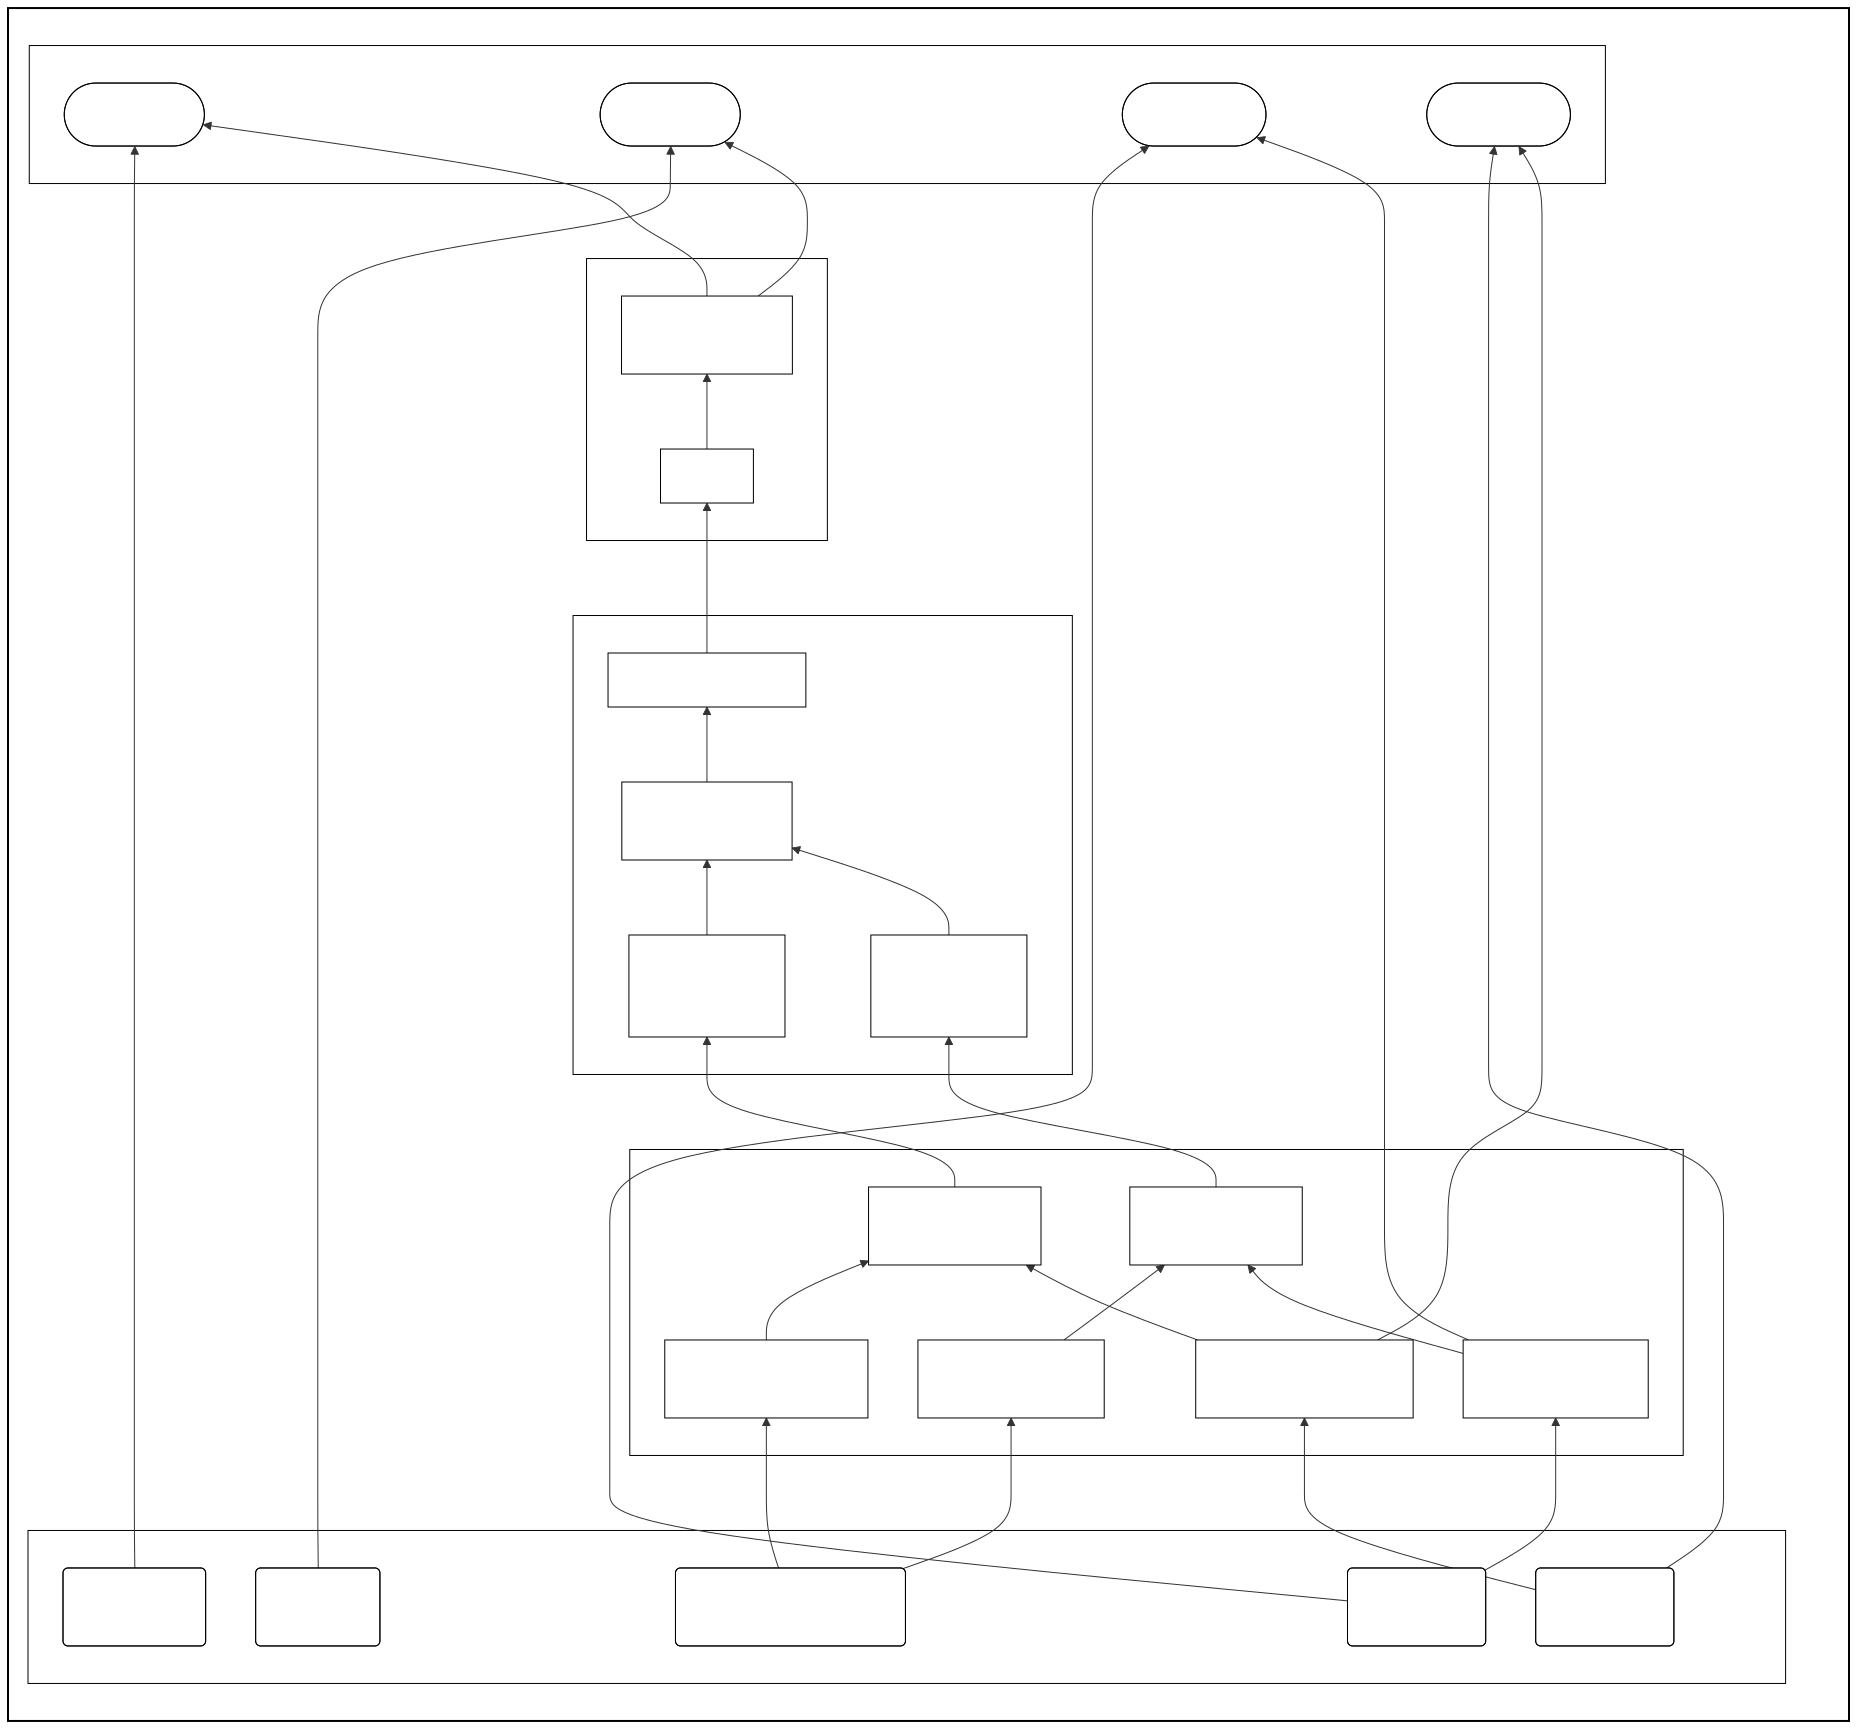
\includegraphics[width=1.0\textwidth]{img/idkt_arch.png}
    \caption{The iDKT Architecture. The diagram illustrates the five functional stages: (1) Input Data ingestion including BKT targets, (2) Individualized Embeddings, (3) the Transformer Core, (4) the MLP-based Output, and (5) the Loss Functions for representational grounding.\label{idkt_arch}}
\end{figure}


\section{Embeddings} \label{sec_embeddings}

In standard educational datasets, such as ASSISTments 2009, ASSISTments 2015, Algebra 2005, and others \citep{liu2022pykt}, student interactions are recorded at the level of specific questions or tasks, each of which is associated with one or more underlying concepts or knowledge components. This structure reflects the fact that proficiency in a concept (e.g., the Pythagorean Theorem) is acquired through interactions with a diverse range of tasks. While all tasks involving a concept share the same semantic core, they differ in their specific manifestations—most notably in their intrinsic difficulty or complexity. Therefore, an effective representation must capture both the shared identity of the concept and the unique deviation of the specific task.

In Transformer-based models \citep{vaswani2017attention} we can operationalize this principle representing the tasks as embedding vectors: 

\begin{equation}
    x' = c + u \cdot d \quad \text{(Task)}
\end{equation}


In this formulation, $c$ acts as the \textit{Concept Anchor}, a vector representing the invariant semantic identity of the concept while the vector $d$ represents the learnable \textit{Question Variation Axis}, defining the specific direction of the "transition gap". The scalar $u$ serves as the \textit{Relational Magnitude}, representing the question's specific relative difficulty compared to other questions involving the same concept. Consequently, rather than encode arbitrary embeddings for every question, we encode the vector sum of two distinct components with clear semantic meaning: a base \textit{concept identity} and a \textit{difficulty shift}. 

In a similar way, we can operationalize the interactions between questions and students as embedding vectors: 

\begin{equation}
    y' = e + u \cdot (f + d) \quad \text{(Interaction History)}
\end{equation}

Here $e$ represents the \textit{Interaction Base}, which is a combined representation of concept c and the binary outcome r (correct/incorrect), while $f$ represents the \textit{Interaction Variation Axis}, which is similar to the Question Variation Axis ($d_c$) but is specific to the interaction between a question and a student. The inclusion of $d_c$ in the interaction shift ensures that the difficulty vectors are consistent across both questions ($x'$) and interactions ($y'$).

Extending this rationale, we can enrich the $x'$ embeddings by integrating additional components with explicit semantic significance. Specifically, by adopting Bayesian Knowledge Tracing (BKT) as a reference model, we can incorporate vectors corresponding to its core theoretical parameters—Initial Knowledge ($L_0$) and Learning Rate ($T$)—thereby grounding the deep representation in established pedagogical constructs. 

To get individualized values for these parameters, we decompose them into population-level bases and student-specific deviations: 

\begin{equation}
    l_c = L_{0} + k_s \cdot d_{k} \quad \text{(Personalized Initial Knowledge)}
\end{equation}
\begin{equation}
    t_c = T + v_s \cdot d_{v} \quad \text{(Personalized Learning Rate)}
\end{equation}


where $l_c$ is the personalized initial knowledge for concept, $t_c$ is the personalized learning rate for concept, $L_{0}$ and $T$ are the population-level base embeddings, $d_{k}$ and $d_{v}$ are the learnable variation axes vectors (similar to the difficulty axis $d$), and $k_s$ and $v_s$ are the scalar student-specific deviations learned for each individual.

We include these vectors to get the final input embedding for the encoder and decoder components of the Transformer: 
\begin{equation}
    x' = (c + u \cdot d) - l_c \quad \text{(Individualized Task)}
\end{equation}
\begin{equation}
    y' = (e + u \cdot (f + d)) + t_c \quad \text{(Individualized Interaction History)}
\end{equation}

where $c$ represents the concept embedding, $u$ the question-specific difficulty shift, $d$ the task variation axis, $e$ the interaction base, $f$ the interaction variation axis, $l_c$ the personalized initial knowledge, and $t_c$ the personalized learning rate.

The rationale for using difference for the individualized task ($x'$) and sum for the interaction history ($y'$) is due to their distinct semantic roles:
\begin{itemize}
    \item $x'$ represents the $\textit{Transition Gap}$: $\textit {Difficulty} - \textit{Proficiency}$. Under this relational logic, objective task difficulty is offset by prior proficiency, ensuring that task demands are defined relative to the subject's baseline. This formulation captures the difference between the task requirements and the current state, representing the residual gap after accounting for latent proficiency.
    \item $y'$ represents the $\textit{Transition Gain}$: $\textit{Interaction} + \textit{Rate}$. The history encoder accumulates evidence from interactions, applying a consistent relational logic where the signal value is augmented by latent rate, ensuring that interaction outcomes are defined relative to the subject's pace. Under this formulation, the total value encompasses not only the interaction outcome but also the rate of progress through the state trajectory, as this incremental gain serves as a robust indicator of future performance. This approach, therefore, captures latent progression by augmenting observed outcomes with transition rate, thereby reflecting individualized acquisition rates.
\end{itemize}

\section{Loss Functions} \label{sec_loss}

The model is trained using a multi-objective loss function designed to ensure that the high-capacity Transformer remains aligned with pedagogical principles through Representational Grounding. The total loss $\mathcal{L}_{total}$ is defined as a weighted sum of different loss components described in detail below. 
\begin{equation}
    \mathcal{L}_{total} = L_{sup} + \lambda_{ref} L_{ref} + \lambda_{init} L_{init} + \lambda_{rate} L_{rate} + L_{reg}
\end{equation}

\subsection{Supervised Alignment ($L_{sup}$)}
The primary objective $L_{sup}$ uses standard Binary Cross-Entropy (BCE) between the iDKT performance predictions $\hat{y}_t$ and the observed ground truth outcomes $r_t \in \{0, 1\}$. This loss ensures predictive accuracy by minimizing the deviance from observed student behavior:
\begin{equation}
    L_{sup} = -\frac{1}{N} \sum_{t=1}^N [r_t \log(\hat{y}_t) + (1-r_t) \log(1-\hat{y}_t)]
\end{equation}

\subsection{Representational Grounding}
The grounding losses ($L_{ref}, L_{init}, L_{rate}$) use Mean Squared Error (MSE) to anchor deep representations to BKT-derived values. Specifically, $L_{ref}$ forces behavioral predictions to stay close to the theoretical baseline, while $L_{init}$ and $L_{rate}$ ground the individualized parameters $l_c$ and $t_c$ in meaningful educational starting points and acquisition paces, respectively. Instead of arbitrary latent weights, the model's internal states are projected through a sigmoid activation $\sigma(\cdot)$ and compared directly to the reference values:
\begin{align}
    L_{ref} &= \text{MSE}(\hat{y}, p_{BKT}) \\
    L_{init} &= \text{MSE}(\sigma(\bar{l}_c), L0_{BKT}) \\
    L_{rate} &= \text{MSE}(\sigma(\bar{t}_c), T_{BKT})
\end{align}
where $\bar{l}_c$ and $\bar{t}_c$ are the average across the feature dimension of the individualized embeddings for proficiency and rate, respectively. This formulation forces the deep representation to be not only predictive but also semantically consistent with the reference constructs.

\subsection{Inductive Bias Regularization ($L_{reg}$)}
While the grounding losses anchor the global position of the latent space to the BKT parameter estimations, $L_{reg}$ ensures that student-level individualization is \textit{parsimonious}. This loss acts directly on the individualization parameters ($u_q, k_s, v_s$) to ensure that the model only deviates from the theoretical prior when functionally necessary. We apply distinct $L_2$ penalties to the scalar parameters governing variation:
\begin{equation}
    L_{reg} = \lambda_{\text{u}} \sum_{q \in Q} u_q^2 + \lambda_{\text{k}} \sum_{s \in S} k_s^2 + \lambda_{\text{v}} \sum_{s \in S} v_s^2
\end{equation}
where $u_q$ represents item difficulty, $k_s$ is the student-specific knowledge gap, and $v_s$ is the learning rate deviation. This formulation implements a \textit{normal student prior}: the model assumes every subject adheres to the population-level parameters derived from the BKT reference unless their unique interaction history provides sufficient signal to justify the regularization cost. 

\section{Results} \label{sec_experiment}

\subsection{Experimental Setup}
\subsection{Datasets}
\subsection{Models}
\subsection{Research Questions}

The experimental validation of iDKT is guided by the following research questions:

\begin{enumerate}
    \item \textbf{Interpretability Validation (RQ1)}: Is it possible to rigorously validate that a iDKT model, whose representations are grounded in a reference model, actually yields interpretable constructs?
    \item \textbf{Accuracy--Interpretability Trade-Off (RQ2)}: To what extent can deep knowledge tracing models be constrained for interpretability alignment without significantly degrading predictive accuracy?
    \item \textbf{Higher Granularity (RQ3)}: Can the proposed model capture individualized latent factors at a higher level of granularity than the reference model?
\end{enumerate}

\subsection{Interpretability Validation} \label{sec_validation}

To verify that iDKT’s internal representations ($l_c, t_c, u_q$) reflect educational constructs throughout training, we employ a verification framework based on two psychometric hypotheses:

\begin{enumerate}
    \item \textbf{$H_1$: Convergent Validity (Latent Fidelity)}: Pearson correlation between latent projections ($l_c, t_c$) and reference BKT parameters. High alignment proves the model has internalized the theoretical constructs.
    \item \textbf{$H_2$: Predictor Equivalence (Behavioral Alignment)}: Functional substitutability of iDKT parameters into canonical BKT mastery recurrence equations. This ensures factors preserve their causal roles defined by theory.
\end{enumerate}

\subsection{Accuracy--Interpretability Trade-Off} \label{sec_tradeoff}

A key contribution of this work is the systematic exploration of the trade-off between predictive accuracy and theoretical fidelity. By modulating the grounding weight $\lambda_{ref}$ in Equation 7, we identify the Pareto frontier of the model. This allows us to determine the "Inductive Bias Bonus"—points where theoretical grounding acts as a beneficial regularizer that improves generalization—and the point of "Over-Constraint," where excessive adherence to the reference model begins to degrade predictive power.

\subsection{Higher Granularity} \label{sec_granularity}

To address RQ3, we introduce a metric termed \textit{Individualization Volume}, defined as the variance ($\sigma^2$) of the student-specific latent parameters ($l_c, t_c$) across the population for each skill. In the reference BKT model, these parameters are fixed per skill, implying a population variance of zero ($\sigma \approx 0$). Therefore, the ability of iDKT to capture granularity is verified by measuring the magnitude of dispersion in its learned parameter distributions. A significant non-zero variance indicates that the model has successfully identified valid student-specific traits—such as variable learning rates—that are obscured by the population-level averaging of the baseline model. We visualize this by plotting the standard deviation profiles for all knowledge components in the curriculum.

%%%%%%%%%%%%%%%%%%%%%%%%%%%%%%%%%%%%%%%%%%
\section{Plots}\label{sec_plots}
We utilize four key visualizations to support our findings:
\begin{enumerate}
    \item \textbf{Confidence Heatmaps} (\textit{per\_skill\_alignment\_predictions.png}): Support \textbf{RQ1}. A grid of students vs. skills showing regions of agreement (Green) and divergence (Red) between iDKT and BKT, validating that individualization is localized and grounded.
    \item \textbf{Mastery Plot Mosaics} (\textit{mosaic\_top\_students.png}): Supports \textbf{RQ3}. Longitudinal tracking of probability trajectories for individual students. Deviations from the monotonic BKT curve demonstrate the model's granular responsiveness to specific interaction histories.
    \item \textbf{Pareto Frontier} (\textit{idkt\_pareto\_frontier.png}): Supports \textbf{RQ2}. A scatter plot of Predictive Accuracy (AUC) vs. Theoretical Fidelity ($r$) across varying $\lambda$ weights, identifying the optimal trade-off point.
    \item \textbf{Correlation Plots} (\textit{per\_skill\_correlation\_predictions.png}): Supports \textbf{RQ1}. Bar charts of parameter correlation per skill, statistically quantifying the degree of semantic alignment ($H_1$).
\end{enumerate}



%%%%%%%%%%%%%%%%%%%%%%%%%%%%%%%%%%%%%%%%%%
\section{Results}\label{sec_results}

To evaluate the proposed iDKT model, we conducted a series of experiments across multiple educational datasets. Table 1 summarizes the alignment metrics across different grounding strengths (\(\lambda\)).

We observe consistent \textbf{Convergent Validity (\(M_1\))}, with the correlation between the model's projected initial mastery (\(l_c\)) and the theoretical prior (\(L_0\)) remaining above \(0.96\) throughout the sweep (see Table~\ref{tab1}).

\begin{table}[H] 
%\small % Change table font size
\caption{Construct Validity and Performance across the Grounding Spectrum.\label{tab1}}
%\isPreprints{\centering}{} % Only used for preprints
\begin{tabularx}{\textwidth}{lcccc}
\toprule
\textbf{Grounding Strength ($\lambda$)} & \textbf{Test AUC} & \textbf{$M_1$} & \textbf{$M_2$} & \textbf{$M_3$} \\
\midrule
0.00 (Baseline) & 0.8317 & 0.9993 & 0.2652 & -0.0325 \\
\textbf{0.10} & \textbf{0.8322} & \textbf{0.9838} & \textbf{0.2949} & \textbf{-0.0330} \\
0.30 & 0.7984 & 0.9691 & 0.3192 & -0.0330 \\
0.50 & 0.7740 & 0.9884 & 0.2828 & -0.0331 \\
\bottomrule
\end{tabularx}
\end{table}

We observe consistent \textbf{Convergent Validity (\(M_1\))}, with the correlation between the model's projected initial mastery (\(l_c\)) and the theoretical prior (\(L_0\)) remaining above \(0.96\) throughout the sweep. This confirms that the Representational Grounding mechanism successfully anchors the deep latent space to the reference theory. Furthermore, the \textbf{Discriminant Validity (\(M_3\))} remains stable at \(r \approx -0.03\), proving that the model successfully disentangles ``Student Knowledge Gap'' (\(k_c\)) from ``Student Learning Velocity'' (\(v_s\)) as distinct, non-redundant traits.

\subsection{Pareto Curve Analysis} \label{sec_pareto}

Our analysis reveals a non-linear trade-off between predictive accuracy and theoretical fidelity. Contrary to the common assumption that interpretability imposes a performance penalty, we identified an \textbf{``Inductive Bias Bonus''} at moderate grounding levels (\(\lambda \approx 0.10\)).

As shown in Table~\ref{tab1}, the model with \(\lambda=0.10\) achieves a Test AUC of \textbf{0.8322}, slightly outperforming the unconstrained baseline (0.8317). This suggests that the BKT-based regularization acts as a beneficial inductive bias, preventing the Transformer from overfitting to noise in sparse interaction histories. However, excessive grounding (\(\lambda > 0.30\)) leads to a sharp decline in predictive performance as the model becomes over-constrained by the simplicity of the reference theory.

\subsection{Granularity of Individualization} \label{sec_granularity}

While standard BKT assigns a fixed ``Learning Rate'' (\(T\)) to all students for a given skill, iDKT captures a rich distribution of \textbf{Individualized Learning Velocities} (\(t_s\)). Figure~\ref{fig_placeholder1} illustrates this ``Delta Distribution'' (\(\Delta = t_s - T\)). We observe a visible right-skewed variance, indicating that for many skills, the Deep Learning model identifies ``fast-track'' learning trajectories that classical population-level models underestimate. This granularity allows for \textbf{Precise Diagnostic Placement}, distinguishing between students who lack initial knowledge (\textit{low} \(l_c\)) versus those who suffer from slow acquisition pace (\textit{low} \(t_s\)).

\subsection{Longitudinal Mastery Dynamics} \label{sec_longitudinal}

The practical impact of these individualized parameters is evident in the mastery analysis. When simulating the mastery acquisition of ``Fast'' vs. ``Slow'' learners on the same sequence of correct responses:
\begin{itemize}
    \item \textbf{Standard BKT} predicts identical mastery curves for both students.
    \item \textbf{iDKT} projects distinct trajectories, where ``Fast'' learners reach the 95\% mastery threshold significantly earlier (fewer interactions) than ``Slow'' learners.
\end{itemize}

This ``Informed Divergence'' validates that iDKT does not merely mimic BKT labels but leverages its transformer core to dynamically adjust the \textbf{Velocity of Mastery} based on the student's historical profile, enabling truly adaptive pacing in intelligent tutoring scenarios.


%%%%%%%%%%%%%%%%%%%%%%%%%%%%%%%%%%%%%%%%%%
\section{Discussion}\label{sec_discussion}

Authors should discuss the results and how they can be interpreted from the perspective of previous studies and of the working hypotheses. The findings and their implications should be discussed in the broadest context possible. Future research directions may also be highlighted.

%%%%%%%%%%%%%%%%%%%%%%%%%%%%%%%%%%%%%%%%%%
\section{Conclusions}\label{sec_conclusions}

This section is not mandatory, but can be added to the manuscript if the discussion is unusually long or complex.

%%%%%%%%%%%%%%%%%%%%%%%%%%%%%%%%%%%%%%%%%%
\section{Patents}

This section is not mandatory, but may be added if there are patents resulting from the work reported in this manuscript.

%%%%%%%%%%%%%%%%%%%%%%%%%%%%%%%%%%%%%%%%%%
\vspace{6pt} 

%%%%%%%%%%%%%%%%%%%%%%%%%%%%%%%%%%%%%%%%%%
%% optional
%\supplementary{The following supporting information can be downloaded at:  \linksupplementary{s1}, Figure S1: title; Table S1: title; Video S1: title.}

% Only for journal Methods and Protocols:
% If you wish to submit a video article, please do so with any other supplementary material.
% \supplementary{The following supporting information can be downloaded at: \linksupplementary{s1}, Figure S1: title; Table S1: title; Video S1: title. A supporting video article is available at doi: link.}

% Only used for preprtints:
% \supplementary{The following supporting information can be downloaded at the website of this paper posted on \href{https://www.preprints.org/}{Preprints.org}.}

% Only for journal Hardware:
% If you wish to submit a video article, please do so with any other supplementary material.
% \supplementary{The following supporting information can be downloaded at: \linksupplementary{s1}, Figure S1: title; Table S1: title; Video S1: title.\vspace{6pt}\\
%\begin{tabularx}{\textwidth}{lll}
%\toprule
%\textbf{Name} & \textbf{Type} & \textbf{Description} \\
%\midrule
%S1 & Python script (.py) & Script of python source code used in XX \\
%S2 & Text (.txt) & Script of modelling code used to make Figure X \\
%S3 & Text (.txt) & Raw data from experiment X \\
%S4 & Video (.mp4) & Video demonstrating the hardware in use \\
%... & ... & ... \\
%\bottomrule
%\end{tabularx}
%}

%%%%%%%%%%%%%%%%%%%%%%%%%%%%%%%%%%%%%%%%%%
\authorcontributions{For research articles with several authors, a short paragraph specifying their individual contributions must be provided. The following statements should be used ``Conceptualization, X.X. and Y.Y.; methodology, X.X.; software, X.X.; validation, X.X., Y.Y. and Z.Z.; formal analysis, X.X.; investigation, X.X.; resources, X.X.; data curation, X.X.; writing---original draft preparation, X.X.; writing---review and editing, X.X.; visualization, X.X.; supervision, X.X.; project administration, X.X.; funding acquisition, Y.Y. All authors have read and agreed to the published version of the manuscript.'', please turn to the  \href{http://img.mdpi.org/data/contributor-role-instruction.pdf}{CRediT taxonomy} for the term explanation. Authorship must be limited to those who have contributed substantially to the work~reported.}

\funding{Please add: ``This research received no external funding'' or ``This research was funded by NAME OF FUNDER grant number XXX.'' and  and ``The APC was funded by XXX''. Check carefully that the details given are accurate and use the standard spelling of funding agency names at \url{https://search.crossref.org/funding}, any errors may affect your future funding.}

\institutionalreview{In this section, you should add the Institutional Review Board Statement and approval number, if relevant to your study. You might choose to exclude this statement if the study did not require ethical approval. Please note that the Editorial Office might ask you for further information. Please add “The study was conducted in accordance with the Declaration of Helsinki, and approved by the Institutional Review Board (or Ethics Committee) of NAME OF INSTITUTE (protocol code XXX and date of approval).” for studies involving humans. OR “The animal study protocol was approved by the Institutional Review Board (or Ethics Committee) of NAME OF INSTITUTE (protocol code XXX and date of approval).” for studies involving animals. OR “Ethical review and approval were waived for this study due to REASON (please provide a detailed justification).” OR “Not applicable” for studies not involving humans or animals.}

\informedconsent{Any research article describing a study involving humans should contain this statement. Please add ``Informed consent was obtained from all subjects involved in the study.'' OR ``Patient consent was waived due to REASON (please provide a detailed justification).'' OR ``Not applicable'' for studies not involving humans. You might also choose to exclude this statement if the study did not involve humans.

Written informed consent for publication must be obtained from participating patients who can be identified (including by the patients themselves). Please state ``Written informed consent has been obtained from the patient(s) to publish this paper'' if applicable.}

\dataavailability{We encourage all authors of articles published in MDPI journals to share their research data. In this section, please provide details regarding where data supporting reported results can be found, including links to publicly archived datasets analyzed or generated during the study. Where no new data were created, or where data is unavailable due to privacy or ethical restrictions, a statement is still required. Suggested Data Availability Statements are available in section ``MDPI Research Data Policies'' at \url{https://www.mdpi.com/ethics}.} 

%\durcstatement{Current research is limited to the [please insert a specific academic field, e.g., XXX], which is beneficial [share benefits and/or primary use] and does not pose a threat to public health or national security. Authors acknowledge the dual-use potential of the research involving xxx and confirm that all necessary precautions have been taken to prevent potential misuse. As an ethical responsibility, authors strictly adhere to relevant national and international laws about DURC. Authors advocate for responsible deployment, ethical considerations, regulatory compliance, and transparent reporting to mitigate misuse risks and foster beneficial outcomes.}

% Only for journal Nursing Reports
%\publicinvolvement{Please describe how the public (patients, consumers, carers) were involved in the research. Consider reporting against the GRIPP2 (Guidance for Reporting Involvement of Patients and the Public) checklist. If the public were not involved in any aspect of the research add: ``No public involvement in any aspect of this research''.}
%
%% Only for journal Nursing Reports
%\guidelinesstandards{Please add a statement indicating which reporting guideline was used when drafting the report. For example, ``This manuscript was drafted against the XXX (the full name of reporting guidelines and citation) for XXX (type of research) research''. A complete list of reporting guidelines can be accessed via the equator network: \url{https://www.equator-network.org/}.}
%
%% Only for journal Nursing Reports
%\useofartificialintelligence{Please describe in detail any and all uses of artificial intelligence (AI) or AI-assisted tools used in the preparation of the manuscript. This may include, but is not limited to, language translation, language editing and grammar, or generating text. Alternatively, please state that “AI or AI-assisted tools were not used in drafting any aspect of this manuscript”.}

\acknowledgments{In this section you can acknowledge any support given which is not covered by the author contribution or funding sections. This may include administrative and technical support, or donations in kind (e.g., materials used for experiments). Where GenAI has been used for purposes such as generating text, data, or graphics, or for study design, data collection, analysis, or interpretation of data, please add “During the preparation of this manuscript/study, the author(s) used [tool name, version information] for the purposes of [description of use]. The authors have reviewed and edited the output and take full responsibility for the content of this publication.”}

\conflictsofinterest{Declare conflicts of interest or state ``The authors declare no conflicts of interest.'' Authors must identify and declare any personal circumstances or interest that may be perceived as inappropriately influencing the representation or interpretation of reported research results. Any role of the funders in the design of the study; in the collection, analyses or interpretation of data; in the writing of the manuscript; or in the decision to publish the results must be declared in this section. If there is no role, please state ``The funders had no role in the design of the study; in the collection, analyses, or interpretation of data; in the writing of the manuscript; or in the decision to publish the results''.} 

%%%%%%%%%%%%%%%%%%%%%%%%%%%%%%%%%%%%%%%%%%
%% Optional

%% Only for journal Encyclopedia
%\entrylink{The Link to this entry published on the encyclopedia platform.}

\abbreviations{Abbreviations}{
The following abbreviations are used in this manuscript:
\\

\noindent 
\begin{tabular}{@{}ll}
MDPI & Multidisciplinary Digital Publishing Institute\\
DOAJ & Directory of open access journals\\
TLA & Three letter acronym\\
LD & Linear dichroism
\end{tabular}
}

%%%%%%%%%%%%%%%%%%%%%%%%%%%%%%%%%%%%%%%%%%
%% Optional
\appendixtitles{no} % Leave argument "no" if all appendix headings stay EMPTY (then no dot is printed after "Appendix A"). If the appendix sections contain a heading then change the argument to "yes".
\appendixstart
\appendix
\section[\appendixname~\thesection]{}
\subsection[\appendixname~\thesubsection]{}
The appendix is an optional section that can contain details and data supplemental to the main text---for example, explanations of experimental details that would disrupt the flow of the main text but nonetheless remain crucial to understanding and reproducing the research shown; figures of replicates for experiments of which representative data are shown in the main text can be added here if brief, or as Supplementary Data. Mathematical proofs of results not central to the paper can be added as an appendix.

\begin{table}[H] 
\caption{This is a table caption.\label{tab5}}
%\newcolumntype{C}{>{\centering\arraybackslash}X}
\begin{tabularx}{\textwidth}{CCC}
\toprule
\textbf{Title 1}	& \textbf{Title 2}	& \textbf{Title 3}\\
\midrule
Entry 1		& Data			& Data\\
Entry 2		& Data			& Data\\
\bottomrule
\end{tabularx}
\end{table}

\section[\appendixname~\thesection]{}
All appendix sections must be cited in the main text. In the appendices, Figures, Tables, etc. should be labeled, starting with ``A''---e.g., Figure A1, Figure A2, etc.

%%%%%%%%%%%%%%%%%%%%%%%%%%%%%%%%%%%%%%%%%%
%\isPreprints{} % If the paper is ``preprints'', please uncomment this parenthesis.
%\printendnotes[custom] % Un-comment to print a list of endnotes

\reftitle{References}

% Please provide either the correct journal abbreviation (e.g. according to the “List of Title Word Abbreviations” http://www.issn.org/services/online-services/access-to-the-ltwa/) or the full name of the journal.
% Citations and References in Supplementary files are permitted provided that they also appear in the reference list here. 

%=====================================
% References, variant A: external bibliography
%=====================================
%\bibliographystyle{Definitions/mdpi}
\bibliography{biblio}

%=====================================
% References, variant B: internal bibliography (commented out)
%=====================================

% ACS format
% \isAPAandChicago{}{%
% \begin{thebibliography}{999}
% % Reference 1
% \bibitem[Author1(year)]{ref-journal}
% Author~1, T. The title of the cited article. {\em Journal Abbreviation} {\bf 2008}, {\em 10}, 142--149.
% ... (truncated for chunk)

% % Chicago format (Used for journal: arts, genealogy, histories, humanities, jintelligence, laws, literature, religions, risks, socsci)
% \isChicagoStyle{%
% \begin{thebibliography}{999}
% % Reference 1
% \bibitem[Aranceta-Bartrina(1999a)]{ref-journal}
% Aranceta-Bartrina, Javier. 1999a. Title of the cited article. \textit{Journal Title} 6: 100--10.
% % Reference 2
% \bibitem[Aranceta-Bartrina(1999b)]{ref-book1}
% Aranceta-Bartrina, Javier. 1999b. Title of the chapter. In \textit{Book Title}, 2nd ed. Edited by Editor 1 and Editor 2. Publication place: Publisher, vol. 3, pp. 54–96.
% % Reference 3
% \bibitem[Baranwal and Munteanu {[1921]}(1955)]{ref-book2}
% Baranwal, Ajay K., and Costea Munteanu. 1955. \textit{Book Title}. Publication place: Publisher, pp. 154--96. First published 1921 (op-tional).
% % Reference 4
% \bibitem[Berry and Smith(1999)]{ref-thesis}
% Berry, Evan, and Amy M. Smith. 1999. Title of Thesis. Level of Thesis, Degree-Granting University, City, Country. Identifi-cation information (if available).
% % Reference 5
% \bibitem[Cojocaru et al.(1999)]{ref-unpublish}
% Cojocaru, Ludmila, Dragos Constatin Sanda, and Eun Kyeong Yun. 1999. Title of Unpublished Work. \textit{Journal Title}, phrase indicating stage of publication.
% % Reference 6
% \bibitem[Driver et al.(2000)]{ref-proceeding}
% Driver, John P., Steffen Rohrs, and Sean Meighoo. 2000. Title of Presentation. In \textit{Title of the Collected Work} (if available). Paper presented at Name of the Conference, Location of Conference, Date of Conference.
% % Reference 7
% \bibitem[Harwood(2008)]{ref-url}
% Harwood, John. 2008. Title of the cited article. Available online: URL (accessed on Day Month Year).
% \end{thebibliography}
% }{}
% 
% % APA format (Used for journal: admsci, behavsci, businesses, econometrics, economies, education, ejihpe, games, humans, ijfs, journalmedia, jrfm, languages, psycholint, publications, tourismhosp, youth)
% \isAPAStyle{%
% \begin{thebibliography}{999}
% % Reference 1
% \bibitem[\protect\citeauthoryear{Azikiwe \BBA\ Bello}{{2020a}}]{ref-journal}
% Azikiwe, H., \& Bello, A. (2020a). Title of the cited article. \textit{Journal Title}, \textit{Volume}(Issue), 
% Firstpage--Lastpage/Article Number.
% % Reference 2
% \bibitem[\protect\citeauthoryear{Azikiwe \BBA\ Bello}{{2020b}}]{ref-book1}
% Azikiwe, H., \& Bello, A. (2020b). \textit{Book title}. Publisher Name.
% % Reference 3
% \bibitem[Davison(1623/2019)]{ref-book2}
% Davison, T. E. (2019). Title of the book chapter. In A. A. Editor (Ed.), \textit{Title of the book: Subtitle} 
% (pp. Firstpage--Lastpage). Publisher Name. (Original work published 1623) (Optional).
% % Reference 4
% \bibitem[Fistek et al.(2017)]{ref-proceeding}
% Fistek, A., Jester, E., \& Sonnenberg, K. (2017, Month Day). Title of contribution [Type of contribution]. Conference Name, Conference City, Conference Country.
% % Reference 5
% \bibitem[Hutcheson(2012)]{ref-thesis}
% Hutcheson, V. H. (2012). \textit{Title of the thesis} [XX Thesis, Name of Institution Awarding the Degree].
% % Reference 6
% \bibitem[Lippincott \& Poindexter(2019)]{ref-unpublish}
% Lippincott, T., \& Poindexter, E. K. (2019). \textit{Title of the unpublished manuscript} [Unpublished manuscript/Manuscript in prepara-tion/Manuscript submitted for publication]. Department Name, Institution Name.
% % Reference 7
% \bibitem[Harwood(2008)]{ref-url}
% Harwood, J. (2008). \textit{Title of the cited article}. Available online: URL (accessed on Day Month Year).
% \end{thebibliography}
% }{}

% If authors have biography, please use the format below
%\section*{Short Biography of Authors}
%\bio
%{\raisebox{-0.35cm}{\includegraphics[width=3.5cm,height=5.3cm,clip,keepaspectratio]{Definitions/author1.pdf}}}
%{\textbf{Firstname Lastname} Biography of first author}
%
%\bio
%{\raisebox{-0.35cm}{\includegraphics[width=3.5cm,height=5.3cm,clip,keepaspectratio]{Definitions/author2.jpg}}}
%{\textbf{Firstname Lastname} Biography of second author}

% For the MDPI journals use author-date citation, please follow the formatting guidelines on http://www.mdpi.com/authors/references
% To cite two works by the same author: \citeauthor{ref-journal-1a} (\citeyear{ref-journal-1a}, \citeyear{ref-journal-1b}). This produces: Whittaker (1967, 1975)
% To cite two works by the same author with specific pages: \citeauthor{ref-journal-3a} (\citeyear{ref-journal-3a}, p. 328; \citeyear{ref-journal-3b}, p.475). This produces: Wong (1999, p. 328; 2000, p. 475)

%%%%%%%%%%%%%%%%%%%%%%%%%%%%%%%%%%%%%%%%%%
%% for journal Sci
%\reviewreports{\\
%Reviewer 1 comments and authors’ response\\
%Reviewer 2 comments and authors’ response\\
%Reviewer 3 comments and authors’ response
%}
%%%%%%%%%%%%%%%%%%%%%%%%%%%%%%%%%%%%%%%%%%
\PublishersNote{}
%\isPreprints{} % If the paper is ``preprints'', please uncomment this parenthesis.
\end{document}

